\documentclass[]{article}
\usepackage{nips13submit_e,times}
\usepackage[utf8x]{inputenc}
\usepackage{amsfonts}
\usepackage{indentfirst}
\usepackage{hyperref}
\usepackage{graphicx}
\usepackage{enumerate}
\usepackage{amsmath}
\usepackage{subfigure}
\usepackage{amsopn}
\title{Project-II by group TORONTO}
\author{Michalina Pacholska \And Jakub Sygnowski}
\nipsfinalcopy


\begin{document}

\section{Persons recognition}
\subsection{Problem and dataset descriptions}
  During the project, we were first given a set images and labels indicating if there is a person. We also were given features extracted from the images and we are supposed to analyze and learn our algorithms only on those extracted features (not on images). Then, a week before the deadline, we were given a test set of features for which we should give our predictions. (Following discussions refer to the train set of features). 

  Our set contains $8545$ images and labels ($1$ - person, $0$ - not), and for every image $9360$ features in a form of a $26\times10\times36$ cube. There are $1237$ images with a person (at least labeled $1$). 

\begin{figure}[!h]
  \center
  \subfigure[picture]{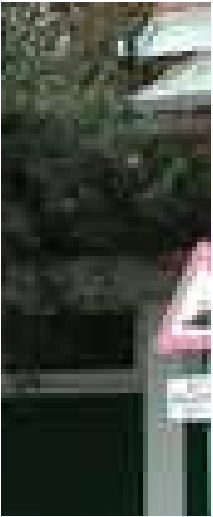
\includegraphics[height=1.7in]{../figures/examplePicture-crop.pdf} \label{fig:examplePicture}}
  \;
  \subfigure[features]{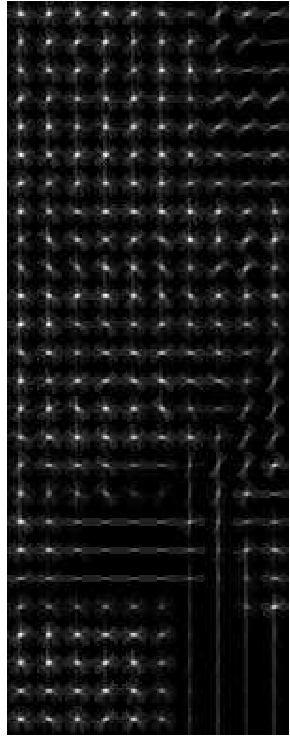
\includegraphics[height=1.7in]{../figures/exampleFeature-crop.pdf} \label{fig:exampleFeature}}
  \caption{ \ref{fig:examplePicture} picture No 200 and \ref{fig:exampleFeature} features extracted form it, using Piotr's toolbox (http://vision.ucsd.edu/~pdollar/toolbox/doc/index.html) %TODO where put this reference
  }
\end{figure}

\subsection{Data analysis and preparation}
  Features first two dimensions $26\times10$ of features for particular image correspond to the position of image form where those features1 were extracted and in the third dimension corresponds to the direction of edges in that part of image. White color and big number indicates that there is the edge, see \ref{fig:examplePicture} and \ref{fig:exampleFeature}. Values of features are between $0$ and $0.2$ and normalization doesn't change them much. 
  \begin{figure}[!h]
  \center
  \subfigure[original data]{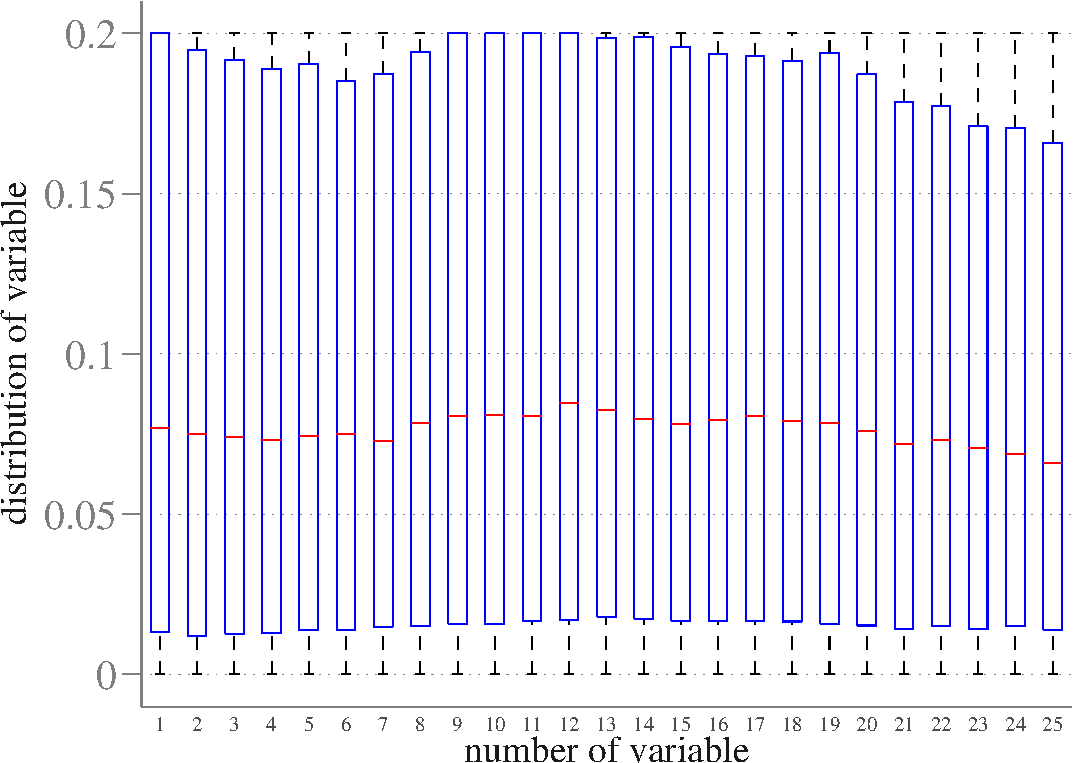
\includegraphics[height=1.8in]{../figures/boxplot1-crop.pdf} \label{fig:boxplot1}}
  \;
  \subfigure[after normalization]{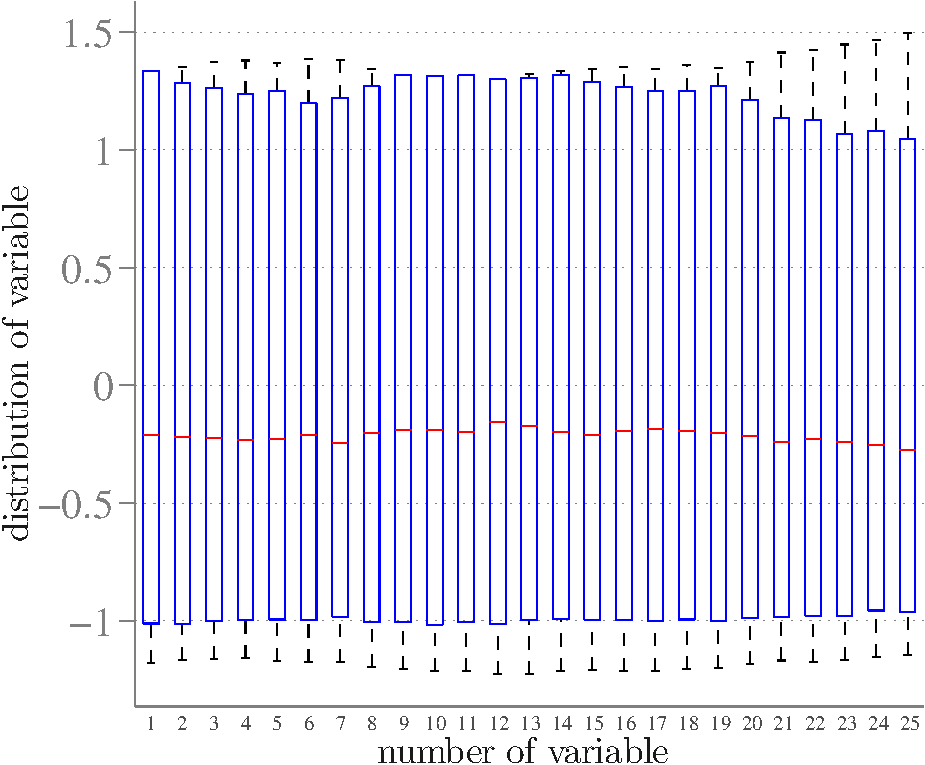
\includegraphics[height=1.8in]{../figures/boxplot2-crop.pdf} \label{fig:boxplot2}}
  \caption{Boxplots of part of the data before \ref{fig:boxplot1} and after \ref{fig:boxplot2} normalization. Rest of the data looks similar.}
\end{figure}
  
  Since there are $9360$ numbers for one picture using all of them will cause overfitting (there is more features than pictures). We calculated correlation of them with output and we obtained picture of abstract person, see \ref{fig:correlation}.
  Also on figure \ref{fig:correlations} we can see that there are regions and gradient more and less important for this task and they have shape of a person. Values of correlation were between $-0.37$ and $0.37$
  \begin{figure}[t]
    \center
    \subfigure[Absolute value of correlation for different directions of gradient]{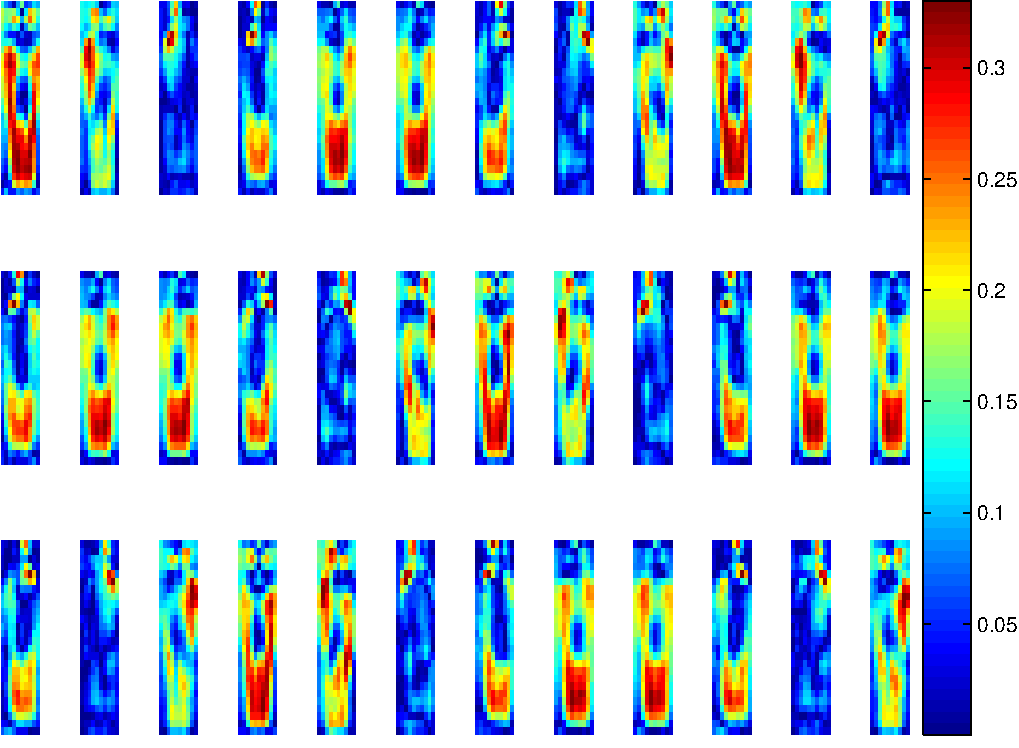
\includegraphics[height=1.7in]{../figures/absoluteCorelation-crop.pdf} \label{fig:correlations}}
      \;\;\;
    \subfigure[positive correlation]{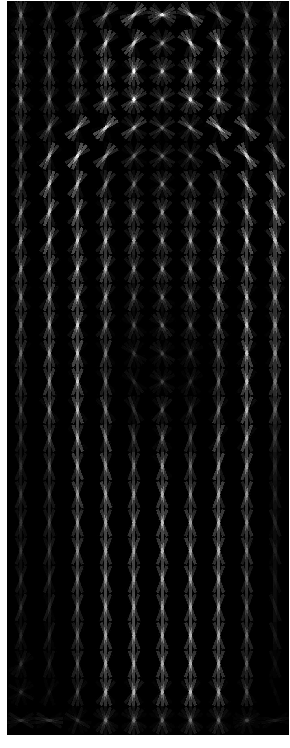
\includegraphics[height=1.7in]		{../figures/averagePerson-crop.pdf} \label{fig:correlation}}
    \caption{Absolute value \ref{fig:correlations} and only positive part \ref{fig:correlation} of correlation, plotted as a feature. There is a lot of not correlated data (deep blue).}
  \end{figure}
  
  Other way of shrinking amount of features is singular value decomposition (i.e. taking only some vectors corresponding to the biggest singular values). That is better idea, because correlation captures only linear dependence and don't see structure in the data. We have done SVD (i.e. we used MatLab's \verb+svds+ function) for $1000$ singular values as a first try and then used $8545\times1000$ as our new feature matrix for testing different methods. 
  
  We planed to do SVD again for bigger numner of singular values, if we will think it's neaded. But then every method we tried was performing better for small number of features (ex. $200$, corresponding to $200$ biggest singular values), in all cases due to variance. So we thought about other way to pick the most significant variables. We used F-score feature selection form libsvm library %TODO cite.
  This method estimate how much for variance of particular variable is correlated to output. We used this method after SVD for two reasons, firstly F-score, the same as correlation, don't encounter structure of the data and second, running F-score on all data needed to much RAM. 
   
% TODO: test matrices descriptions.

\section{Applied methods}
We applied many methods for this task, for most of them we used existing libraries. To check which method is better we were were doing cross-validation and then taking predictions both for train and test into one big vector and passing it as predictions to function \verb+evaluateMultipleMethods+, which was given to us together with data. That was giving us estimate how big is estimate of particular method.

\subsection{Penalized logistic regression}
We started with the the simplest (penalized) logistic regression. Not surprisingly, this method has quite big bias. What's interesting, when we were using $1000$ features (from SVD) it also had big variance. Setting bigger penalty ($\lambda$) caused even bigger bias and very poor performance. Decreasing number of features helped decreasing variance. Penalized logistic regression was working the best with only about $120$ features and $\lambda = 0.1$, and gave average TPR 0.831, see \ref{fig:ROClinear}.

We tried to use most correlated part of all of the data (without decomposition), but to then penalized logistic regression needed more data (and more time) and was performing much poorer. At that point we abandoned using not decomposed data, because we expected that using the most correlated data should be the best suited for simple model like penalized logistic regression.

Then we used data selected by F-score and it improved slightly. We used the same number of variables $120$ and the same $\lambda = 0.1$, which seemed to be the best also in this case. Average TPR was 0.865, see \ref{fig:ROClinear2}.
% [p1,p2,y] = crossValidation(labels(permutacja),U(permutacja,1:120),4,0.1);
  \begin{figure}[h]
    \center
    \subfigure[ROC curves for penalized logistic regression (test and train data) compared with random assignment.]{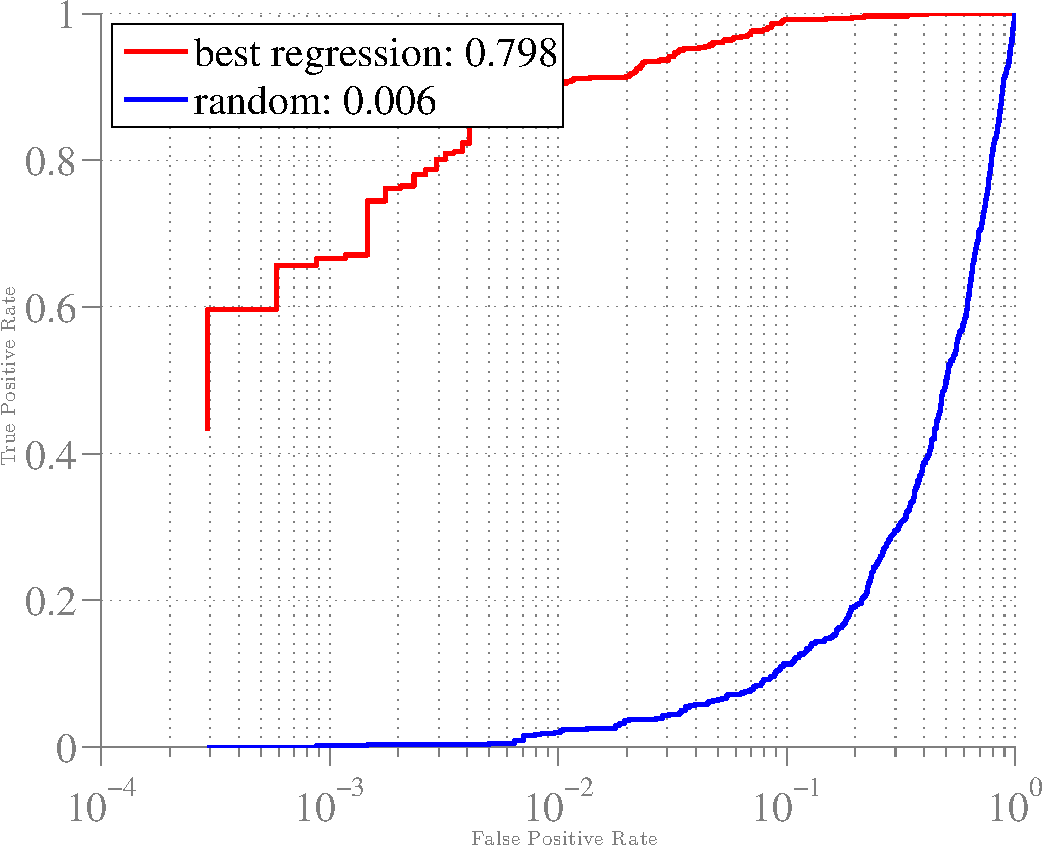
\includegraphics[height=1.7in]{../figures/ROClinear-crop.pdf} \label{fig:ROClinear}}
    \subfigure[ROC curves for penalized logistic regression (test and train data) when using data with the best F-score]{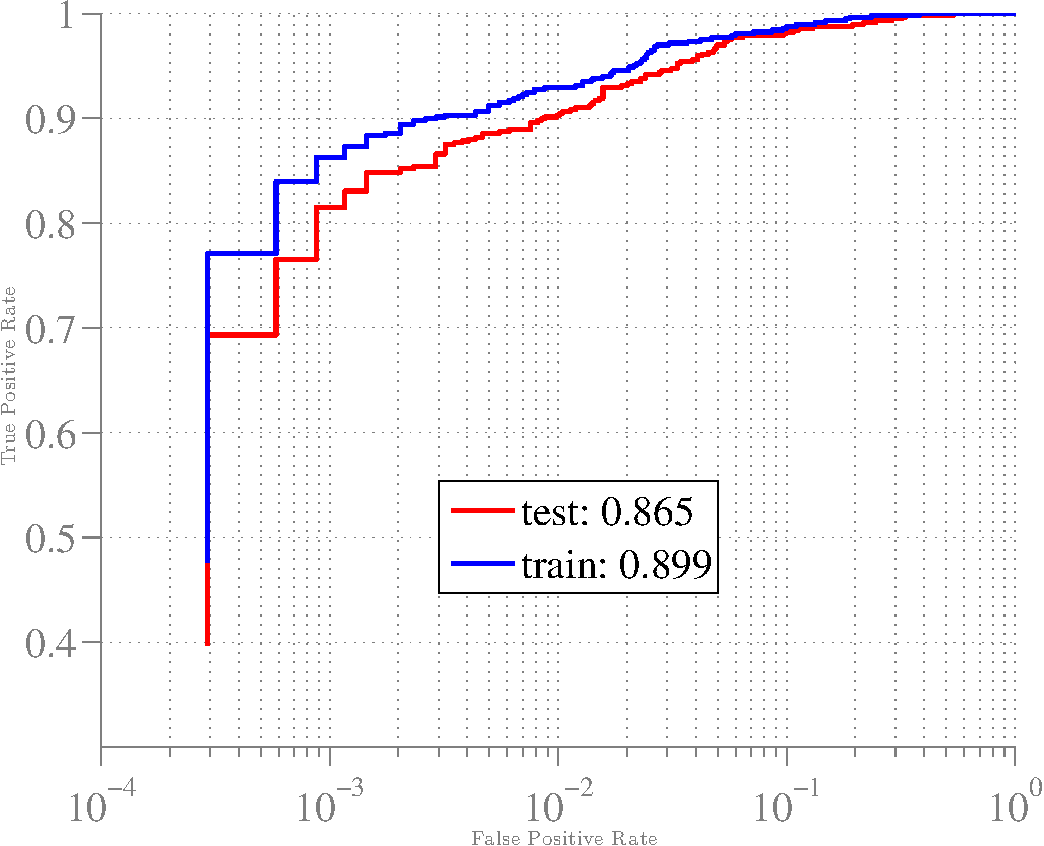
\includegraphics[height=1.7in]{../figures/ROClinear2-crop.pdf} \label{fig:ROClinear2}}
    \caption{ROC curves for two best logistic regression models. \ref{fig:ROClinear2} has better average TPR, but \ref{fig:ROClinear} performs better for small False Positive Rate, what crucial in this task.}
  \end{figure}

\subsection{Support Vector Machine}

For SVM we used svm library. %TODO reference.
We tried different kernels for SVM, but didn't try any custom one. We used built in grid search for parameters of kernel, and then tried to tune them, the last part haven't gave much improvement. More significant was changing amount of variables in the models. We think optimal value was about 120. For all models we obtained similar TPR, about $0.85$, but they didn't managed with small False Positive Rate very well.

  \begin{figure}[h]
    \center
    \subfigure[ROC curves for SVMs, rbf-kernel and linear-kernel.]{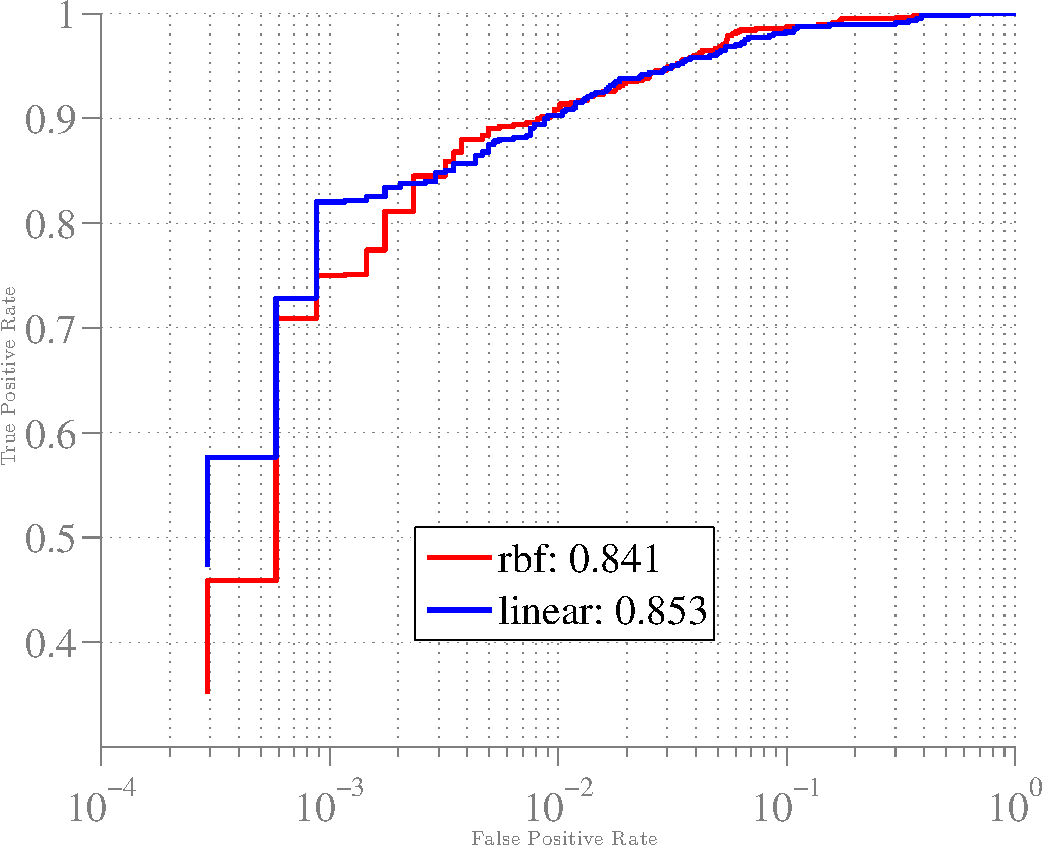
\includegraphics[height=1.7in]{../figures/ROCSVM-crop.pdf} \label{fig:ROCSVM}}
    \subfigure[ROC curves for test and train for SVMs rbf-kernel. It also looks like overfitting]{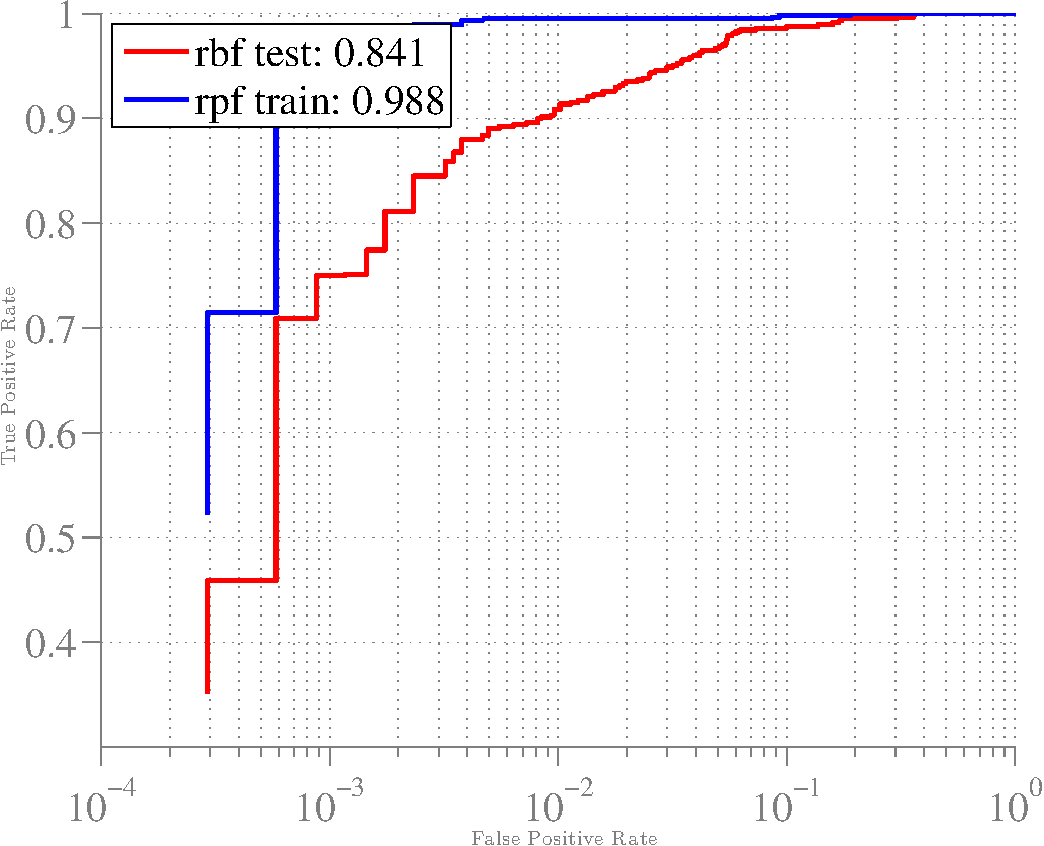
\includegraphics[height=1.7in]{../figures/ROCSVMtrain-crop.pdf} \label{fig:ROCSVM}}
    \caption{ROC curves for SVMs}
  \end{figure}

\subsection{Neural Network}
For Neural Network we used all of the data. We tuned the parameters and obtained the best performance for $2$ layers, first of $50$ hidden variables and second of $2$ hidden variables, see \ref{fig:ROCneural}. We tried to use Neural Network on decomposed matrix, but it was working half that good. It's not surprising, since Neural Network is supposed to capture abstraction from data and SVD may destroyed some structure. But even for Neural Network using $200$ features after SVD was performing better than using $1000$ of them.

  \begin{figure}[h]
    \center
    \subfigure[ROC curves for best tuned Neural Network and random choice.]{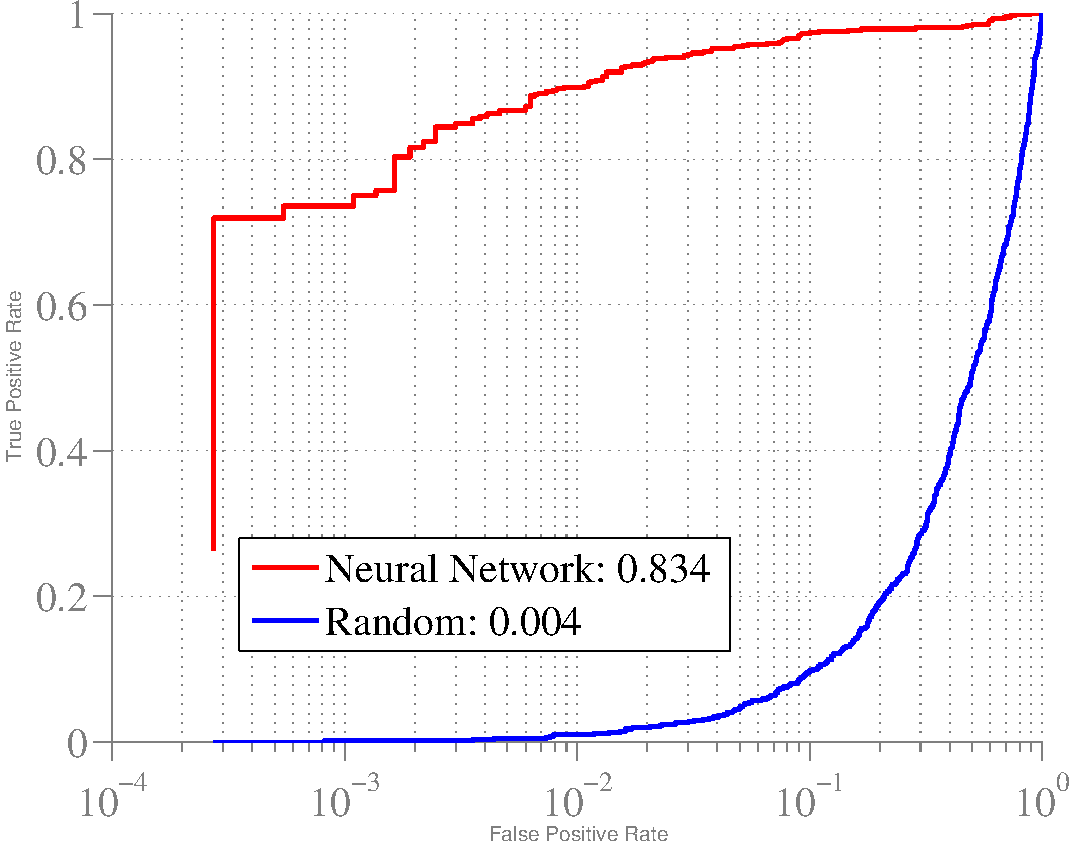
\includegraphics[height=1.7in]{../figures/ROCneural-crop.pdf} \label{fig:ROCneural}}
     \subfigure[ROC curves for test and train for Random Forest for 2000 trees and 100 variables. It looks like random forest is overfitting]{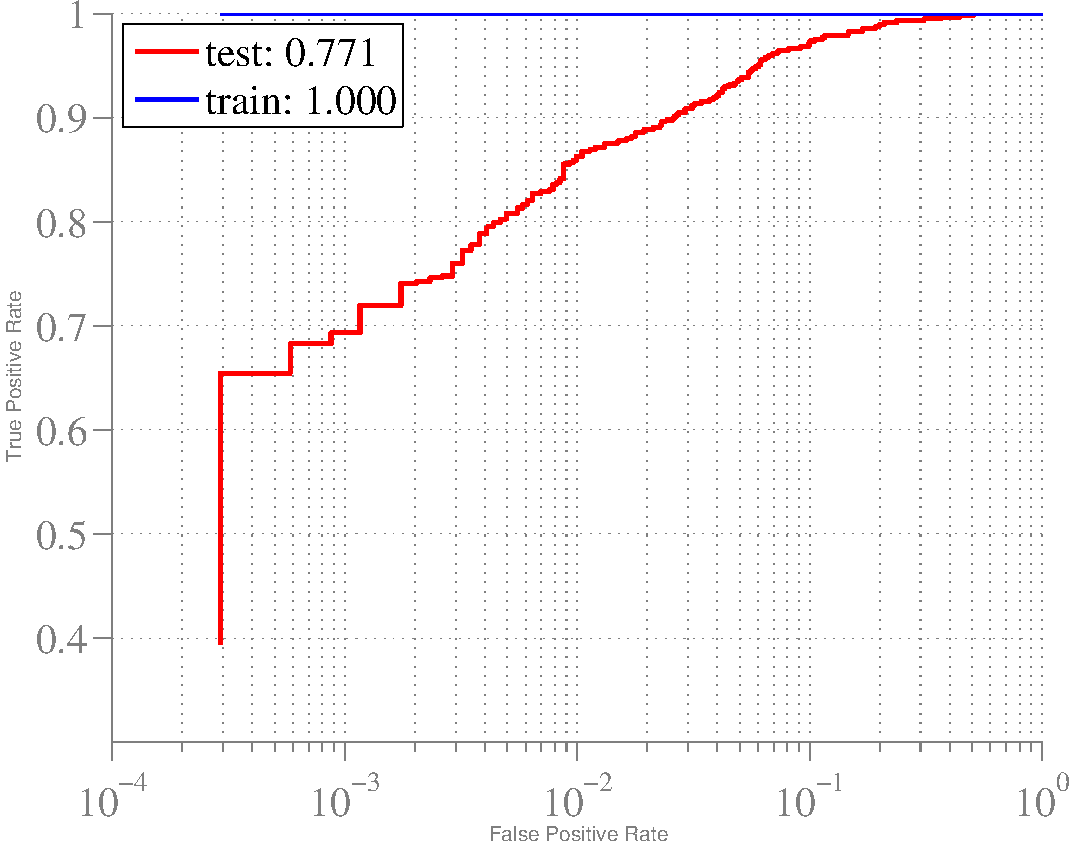
\includegraphics[height=1.7in]{../figures/ROCtree-crop.pdf} \label{fig:ROCtree}}
    \caption{ROC curves for Neural Network \ref{fig:ROCneural} and Random Forest \ref{fig:ROCtree}}
  \end{figure}

\subsection{Random Forest}

For Random Forest we used library %TODO 
We were taking predictions for single trees and averaging them, and treated this average as probability of point belonging to specific class.  
When we were using default number of trees and number of variables sampled in each split (\verb+mtry+), Random Forest suffered form to big variance, even for small amount of data, so we were using it only for d We tried to fix it by increasing number of trees, but it didn't helped much.
We tried also to change \verb+mtry+, but it seamed that default (square root of number of variables) is the best. 

To sum up Random Forest performed poorer than other methods.
We think that it may be good idea to try using Random Forest for choosing most important variables, since it looks like it was the most important thing it this task, but we didn't managed to do this.

\end{document}
